\chapter{Overview of the Dual-Phase Detector Module Design}
\label{ch:fddp-ov}

%%%%%%%%%%%%%%%%%%%%%%%%%%%%%%%%%%%%%%%%%%%%%%%%%%%%%%%%%%%%%%%%%%%%
\section{Description}
\label{sec:fddp-ov-description}

This DUNE-DP design implements a Dual-Phase liquid argon time projection chamber (LArTPC) augmented with a light-readout system. ``Dual-Phase'' refers to the extraction of ionization electrons at the interface between liquid and gas argon and their amplification and collection in the gas phase.

The DUNE-DP module features 12~kTon active mass LArTPC, with all associated cryogenic, electronic readout, computing, and safety systems. The detector is designed to maximize the active volume within the confines of the membrane cryostat while minimizing dead regions and the presence of dead materials in the drift region. The detector is built as a single active volume 60~m long, 12~m wide and 12~m high, with the anode at the top, the cathode near the bottom and an array of photomultiplier (PMTs) located at the bottom of the vessel underneath the cathode. The active volume (see Figure~\ref{fig:DP_det1}) is surrounded by the field cage. The ionization electrons in the liquid phase drift  in a uniform electric field towards the anode plane at the top of the active volume. This is made by an array of 80 independent CRP modules, 3$\times$3~m$^2$ each. The cryogenic front-end electronics is hosted in the signal penetrations (Chimneys) on the roof of the cryostat. There are no active electronics elements in the cryostat volume apart the photomultipliers bases.
The proposed design optimally exploits the cryostat volume of 14(w)$\times$14.1(h)$\times$62(l)~m$^3$ with an anode active area of 12$\times$60~m$^2$ and a drift length of 12~m, corresponding to an active mass of 12.096~kt of LAr (10.643~kt fiducial). 

The detector elements (CRPs and field cage and cathode modules) have been modularized such that their production can proceed in parallel with the construction of the DUNE caverns and cryostats, and sized so that they conform to the access restrictions for transport underground. Table \ref{tab:dune-dp-parameters} summarizes some of the high-level parameters of the DUNE-DP detector while Figure~\ref{fig:DP_det1} shows an overview of the  the Dual-Phase TPC  with its main components.

\begin{dunetable}[DUNE-DP Parameters]{lll}{tab:dune-dp-parameters}{DUNE-DP Parameters}
Parameter & Value & Note \\ \toprowrule
Cryostat LAr Mass & 17.5~kTon & \\
Active LAr Mass & 12.1~kTon & \\ 
Active Height & 12~m & \\ 
Active Length & 60~m & \\ 
Maximum Drift & 12~m & \\ \colhline 
Number of CRPs & 80 & \\ 
Number of CRP Channels & 153,600 & \\
Number of photomultiplier Channels & 720 & \\ \colhline
\end{dunetable}

\begin{dunefigure}[optional caption for LoF]{fig:DP_det1}
{The DUNE Dual-Phase detector with cathode, photomultipliers, field cage and anode plane with signal feedthrough chimneys.}
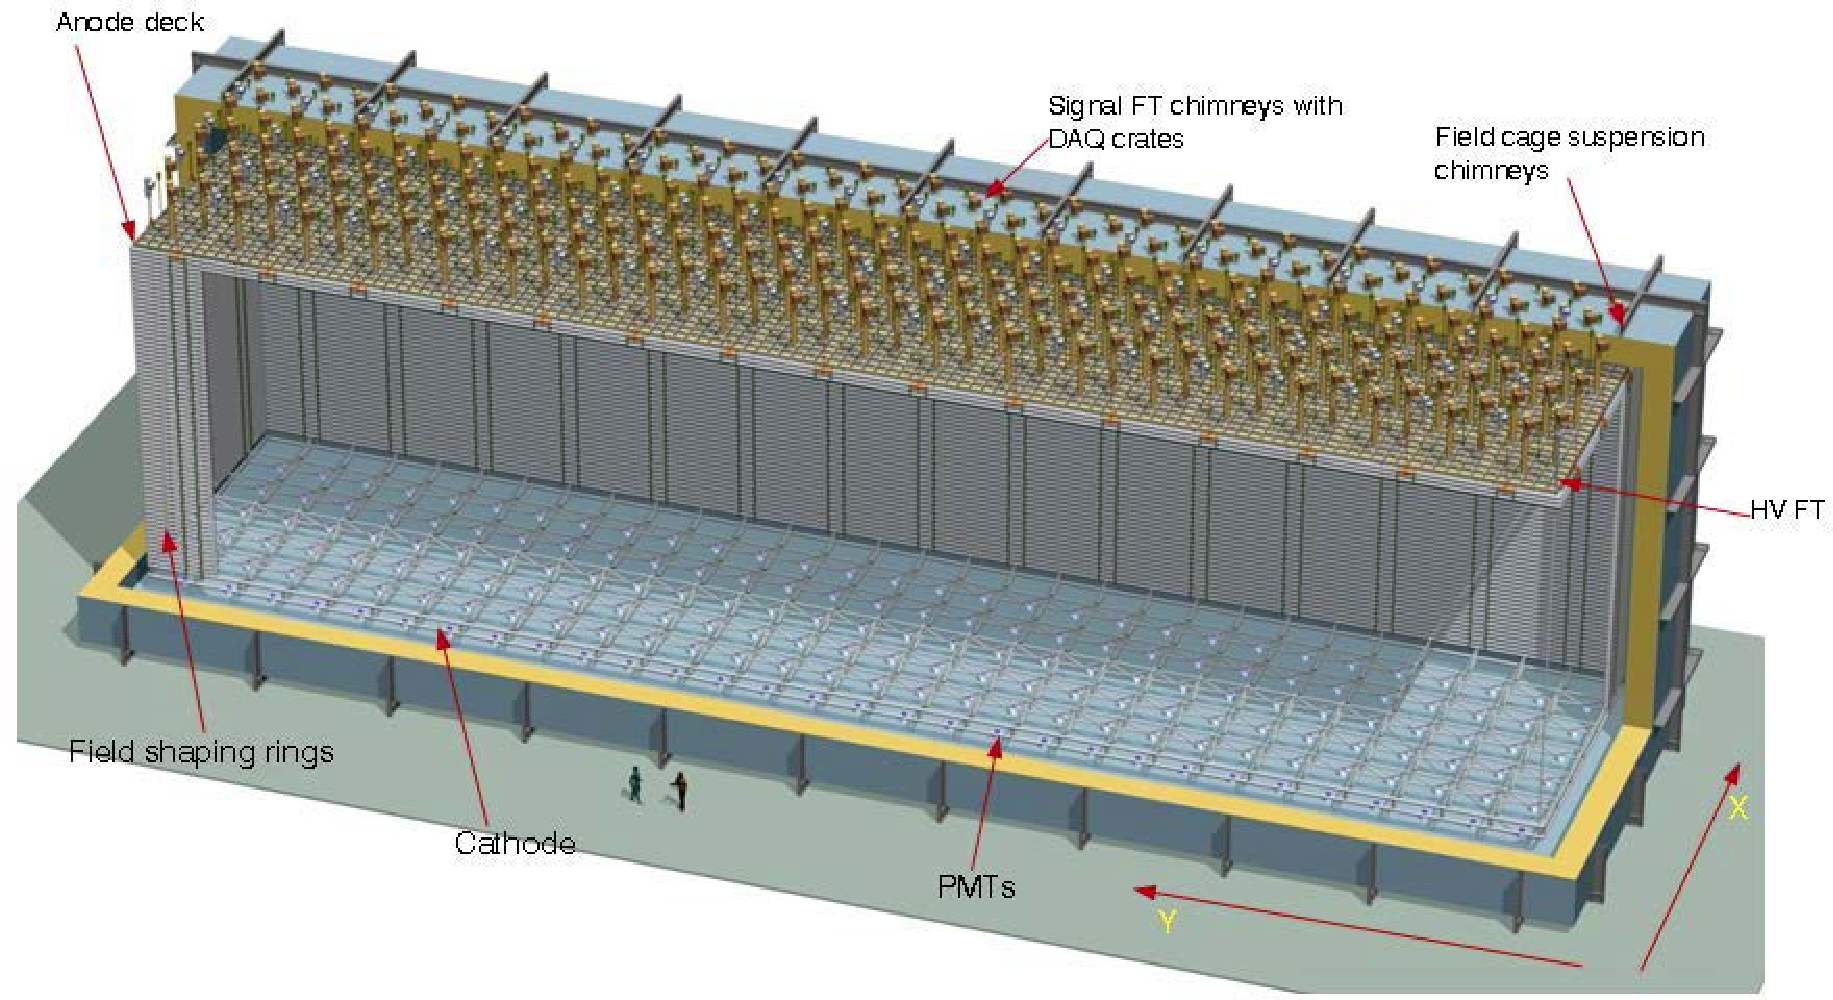
\includegraphics[width=0.8\textwidth]{DUNE-CDR-detectors-volume-optim.pdf}
\end{dunefigure}

The extraction of the electrons from the liquid to vapor phase is performed thanks to the submersed horizontal extraction grid, integrated in each CRP structure. A CRP unit includes 36 (0.5~m$\times$0.5~m) LEM/anode sandwiches, providing tunable amplification and charge collection on two independent views organized in strips of 3-m length and 3.125-mm pitch. There are 1920 readout channels for each CRP. Signals in each CRP unit are collected via three signal feedthrough chimneys hosting the front-end cards with the cryogenic ASIC amplifiers (640 channels/chimney) which are accessible and replaceable without contaminating the pure liquid argon volume. Each chimney is coupled to a microTCA crate ensuring the signals' digitization and 
data acquisition. These crates are connected  via optical fiber links to the DAQ back-end. The total number of readout channel  per \ktadj{10} module is 153,600.

Each CRP unit is independently suspended by three stainless steel ropes. The vertical level of each CRP unit can then be automatically adjusted with respect to the LAr level via three suspension feedthroughs. The stainless steel ropes are operated by step motors which are located outside the suspension feedthroughs. Slow-Control feedthroughs,  one per CRP unit, are used for the signals readout for level meters and the temperature probes, for the pulsing of the calibration signals and to apply the HV bias on the two sides of the LEMs and on the extraction grid. The field cage and the anode are made out of modules of similar dimensions ad in ProtoDUNE-DP.

The number of components and corresponding parameters for the \ktadj{12} dual-phase LArTPC are summarized in Table~\ref{tab:DP_numbers}.

\begin{dunetable}[Quantities of items or parameters for the \ktadj{12}  dual-phase LArTPC]{ll}{tab:DP_numbers}{Quantities of Items or parameters for the \ktadj{12}  dual-phase  LArTPC}  Item & Number or Parameter    \\ \toprowrule
Anode plane size & W = 12~m, L = 60~m \\ \colhline
CRP unit size & W = 3~m, L = 3~m  \\ \colhline
CRP units & 4 $\times$ 20 = 80 \\ \colhline
LEM/Anode sadwiches per CRP unit & 36 \\ \colhline
LEM/Anode sandwiches (total) & 2,880 \\ \colhline
SFT chimneys / CRP unit & 3 \\ \colhline
SFT chimneys (total) & 240 \\ \colhline
Charge readout channels / SFT chimney & 640  \\ \colhline
Charge readout channels (total) & 153,600 \\ \colhline
Suspension FT / CRP unit & 3  \\ \colhline
Suspension FTs (total) & 240  \\ \colhline
Slow Control FT / sub-anode & 1  \\ \colhline
Slow Control FTs (total) & 80 \\ \colhline
HV feedthrough & 1  \\ \colhline
HV for vertical drift & 600~kV \\ \colhline
Voltage degrader resistive chains & 4 \\ \colhline
Cathode modules & 80  \\ \colhline
Field cage rings & 60     \\ \colhline
Field cage ring vertical spacing & 200~mm  \\ \colhline
Field cage resistors (total) & 240    \\ \colhline
Field cage modules & 244  \\ \colhline
PMTs (total) & 720 (1/~m$^2$) \\ 
\end{dunetable}

A number of factors make the dual-phase TPC concept, as described in this chapter, well suited to large detector sizes like the DUNE far detector.
In this design, the charge attenuation on the long drift paths is compensated by the charge amplification in the CRPs.  This configuration also simplifies
construction by optimally exploiting the long vertical dimensions of the cryostat, providing a large homogeneous fiducial volume  free of embedded passive materials (effectively increasing the detector size), reducing the number of readout channels,  and ultimately lowering costs.  

The CRPs collect the charge in a projective way,  with practically no dead region and read the signals out  in two collection views, eliminating the need for  induction views, which  simplifies the reconstruction of complicated topologies. The tunable high S/N provides operative margins with respect to the noise and electron lifetime conditions and lowers the threshold on the minima  detectable energy depositions .

The scope of a dual-phase far detector module for DUNE includes the design, procurement, fabrication, testing, delivery, installation and
commissioning of the detector components which is organized in detector consortia (specific DP consortia or joint SP-DP consortia):

\begin{itemize}
\item Charge-Readout Planes (CRP), including extraction grid, Large Electron Multiplier (LEM) and anode and readout planes (DP consortium);
\item Analog and digital electronics and signal feedthrough chimneys (DP consortium); 
\item Photon detection system (DP Consortium);
\item Cathode, field cage and high voltage system (joint SP-DP consortium);  
\item Slow-Control (joint SP-DP consortium); 
\item Back-end data acquisition system (joint SP-DP consortium).
\end{itemize}

\section{Detector systems}
\label{sec:fddp-ov-systems}

\subsection{Charge Readout Planes}
\label{v4:fddp-ov:crp}

An extraction efficiency of 100\% of the electrons from the liquid to the gas phase is achieved with an electric field of the order of 2~kV/cm across the liquid-gas interface, applied between an  extraction grid submersed in the liquid and charge amplification  devices situated in the ultra-pure argon gas. 

These amplification devices, called Large Electron Multipliers (LEMs), are horizontally  oriented 1-mm-thick printed  circuit boards with electrodes on the top and bottom surfaces. They are drilled through with many holes that collectively form a micro-pattern structure;  when a 3-kV potential difference is applied across the electrodes the ionization electrons are amplified by avalanches (Townsend multiplication) occurring in the  pure argon gas in this micro-pattern structure due to the high electric field (30 kV/cm).

The use of avalanches to amplify the charges in the gas phase increases the S/N ratio by at least one order of magnitude with a typical gain of 20--100, significantly improving the event reconstruction quality. It also lowers the threshold for small energy depositions and provides a better resolution per volumetric pixel (voxel) compared to a Single-Phase LArTPC.  The charge is collected in a finely segmented 2D ($x$ and $y$) readout anode plane at the top of the gas volume and fed to the front-end electronics.   

The  collection, amplification and readout components are combined in an array of independent (layered) modules called Charge Readout Planes (CRPs). A CRP is  composed of several 0.5$\times$0.5-m$^2$ units, each of which is composed  of a LEM/anode sandwich.  These units are embedded in a mechanically reinforced frame of FR-4 and iron-nickel invar alloy. This design guarantees the planarity requirements over the CRP span although the temperature gradient present in the gas phase and possible sagging effects with respect to the three suspension point. The CRP structure also integrates  the submersed extraction grid, which is an array of $x$ and $y$ oriented stainless steel wires, 0.1~mm in diameter, with 3.125-mm pitch. Thicknesses and possible biasing voltages for the different layers are indicated in Figure~\ref{fig:CRP_struct}.

\begin{dunefigure}[optional caption for LoF]{fig:CRP_struct}
{Thicknesses and HV values for electron extraction from liquid to gaseous Ar, their  multiplication by LEMs and their collection on the $x$ and $y$ readout anode plane. The HV values are indicated for a drift field of 0.5~kV/cm in LAr.}
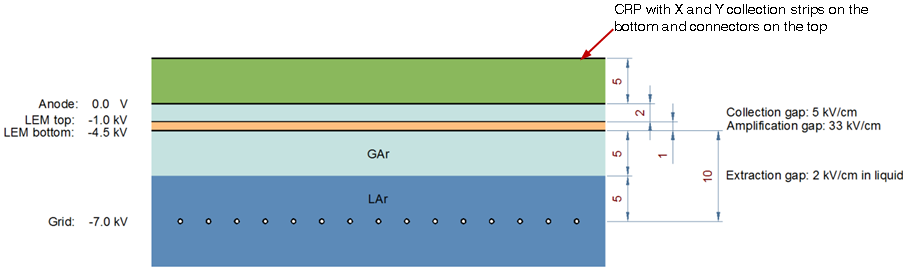
\includegraphics[width=0.8\textwidth]{CRP_gaps.png}
\end{dunefigure}

Each CRP is independently suspended by three stainless-steel ropes linked to the tank top deck. This suspension system allows adjustment of the CRP distance and parallelism with respect to the LAr surface, and keeps the extraction grid immersed. A CRP provides an adjustable charge gain (with a minimal required gain of 20) and two independent, orthogonal readout views, each with a pitch of 3.125~mm.  The LEM/anode sandwiches  in the same CRP unit are interconnected with short flat cables so that each readout channel corresponds to a total strip length of 3~m. Combined with the time information coming from the LAr scintillation readout by the PMT arrays ($t_0$), a CRP provides 3D track imaging with $dE/dx$ information.  The CRPs and their components are described in Chapter~\ref{ch:fddp-CRP}.

The typical amplification achieved by this design, between 20--100, improves the S/N ratio and thus  compensates for the charge losses that occur along the very long drift paths due to the presence of  electronegative impurities. Therefore, despite the longer drift length, this design requires no higher 
purity of the LAr than does the reference design, around 0.1~ppb (or 100~ppt) of oxygen equivalent, and yields a 3-ms electron lifetime. The required level of purity can be reached by starting from  commercially available ppm-level bulk argon and filling a non-evacuated vessel\cite{WA105_TDR}.

The S/N ratio can exceed 100 for a minimum ionizing particle (MIP) after a drift path of 12~m (given an electron lifetime of 3~ms, a drift field of 0.5~kV/cm and a LEM gain of 180). With the same drift field, the same electron-lifetime conditions and a LEM gain of 25, the S/N is larger than 50:1 for tracks up to 6~m from the anode; it reaches 14:1 for MIP tracks that are 12~m from the anode.

Other feedthroughs than the signal chimneys connected to the CRPs and the CRP slow control and feedthroughs are planned for the cathode HV connection, the CRPs' suspension and level adjustment, the high voltage and signal readout of the PMTs, and the monitoring instrumentation (level meters, temperature probes, strain gauges, etc.).


\subsection{Readout electronics and ``Chimneys''}
\label{v4:fddp-ov:electronics}

The electrical signals from the collected charges are passed to the outside of the tank via a set of dedicated signal feedthrough ``chimneys''. The chimneys are pipes passing through the top layer of the cryostat insulation and closed at the top and at the bottom by ultra-high vacuum flanges (warm and cold flange). The volume inside each chimney is tight with respect to the cryostat inner volume and it is filled with nitrogen gas. The bottom (cold) flange of each chimney is at short distance with respect to the CRPs in the cryostat gas volume.

The cryogenic Front-End (FE) electronics cards, housed at the bottom of the chimneys are plugged to the top side of  the cold flange. The FE cards are based on analog cryogenic preamplifiers implemented in CMOS ASIC circuits for high integration and large-scale affordable production. The ASIC circuits have been especially designed, following an R\&D process started in 2006, in order to match the signal dynamics of Dual-Phase. Within the chimneys, the cards are actively cooled to a temperature of about 110 K and isolated with respect to the LAr vessel by the cold flange feedthrough.  The bottom side of the cold flange is connected to the CRP via short flat cables of (0.5~m length) in order to minimize the input capacitance to the preamplifiers. Each chimney collects 640 readout channels. The chimney design allows accessing and replacing the analog front-end electronics from the outside without contaminating the LAr volume since the FE cards are mounted on 2 m long blades sliding on lateral guides integrated in the mechanical structure of the chimneys. Swapping the FE electronics requires opening a flange at the top of the chimney and feeding the chimney with nitrogen in slight over-pressure with respect to the atmospheric pressure.  This operation can be performed while the detector is taking data and it is a quite rapid and straightforward. The chimneys are also Faraday cages and they decouple completely the analog FE electronics with respect to possible noise pickup from the digital electronics.   

The digital electronics for the  charge digitization system is located at warm on the roof the cryostat. This layout makes possible the use of low cost/high speed  networking technologies used in the telecommunication industries such as microTCA. The digital electronics was also developed thanks to a long R\&D process started in 2006.  Digitization cards in the microTCA  Advanced Mezzanine Card (AMC) format read 64 channels/card. Each AMC card can digitize all the 64 channels at 2.5 MHz and compress and transmit this continuous data stream, without zero skipping, over a network link operating at 10 Gbit/s. Lossless data compression is particularly effective thanks to the high S/R of dual phase which limits noise contributions at the level of 1 ADC count. Each signal chimney is coupled to a uTCA crate housing in 10 AMC digitization cards in order to read 640 channels and transmit the data via the  microTCA Carrier Hub (MCH) switch via a 10 Gbit/s optical link connected to the DAQ back-end. 240 uTCA crates are sufficient to read the entire detector module. The chimney warm flange is used to connect the analog differential signals, via shielded VHDCI cables, to the AMC digitization cards and also to distribute the low voltage and slow control signals to the analog FE electronics.  

The light readout digitization system is also based on uTCA AMC cards derived from the design of the charge readout and hosting a specific circuitry, based on the CATIROC ASIC for the light readout triggering. By assuming a PMTs channels density similar as in ProtoDUNE-DP, 5 microTCA crates are sufficient to read 720 PMts.

The timing synchronization is based on the White Rabbit (WR) standard. Specifically developed timing MCH connected to a White Rabbit network ensure the distribution of clock/absolute timing/trigger information on the backplane of the uTCA crates. The WR MCH are connected via 1 Gbit/s optical fibers to a system of WR switches which interconnect the WR network. This ensures that the digitization performed by the various AMC cards is completely aligned and it also connected to the absolute UTC time. The grand-master WR switch is connected to a GPS disciplined oscillator unit providing absolute time and the clock frequency reference to the system. The timing system includes 16 WR switches and 240 (charge readout) + 5 (light readout) MCH units.    

The entire readout electronics system has been optimized in order to cope to the Dual-Phase features including charge signals dynamics, the readout organization via the chimneys, the number of readout channels, the high S/N ratio and the possibility of performing a continuous data streaming with zero losses to the DAQ back-end. The other aspect which has been taken into account since the beginning of the R\&D is the costs reductions and optimization by using particularly cost effective technologies and by performing the corresponding developments in order to fully exploit these technologies.  This optimization adds to the fact that the number of readout channels is naturally lower for a Dual-Phase detector thanks to the long projective geometry: 153600 channels for a DP module with 3 mm readout pitch to be compared to 384000 channels for a SP module with 5 mm readout pitch.

\subsection{Cathode, Field Cage and HV System}
\label{v4:fddp-ov:cathode}

The high voltage system is designed by a common SP-DP consortium.
The drift field (E ${\simeq}$ 0.5~kV/cm) inside the fully active LAr volume is produced by applying high voltage to the cathode plane at the bottom of the cryostat and is kept uniform by the field cage, a stack of 60 equally spaced field-shaping electrodes,  polarized at linearly decreasing voltage from the cathode  voltage to almost ground potential, reached at the level of the charged readout plane. The electrodes are rectangles made of extruded aluminum profiles   (vertical pitch 200~mm) with rounded corners running horizontally (and stacked vertically) around the active volume. The aluminum profiles are supported and insulated by FRP supporting beams with a pattern of slots where the aluminum profiles can be mounted. Similarly as in ProtoDUNE-DP the profiles are arranged in modules of about 3 m size including two FRP supporting columns. These modules are chained together and  are hanging from the cryostat roof. A chain of 12 modules ensured covering 12 m drift. The aluminum profiles of different modules are joined together with specific clips in order to ensure the electrical continuity of the 60 m long horizontal rings.  The drift cage design shares common structure elements (aluminum profiles and FRP supporting beams) as the SP field cage design but with a different arrangement (vertically hung structure) in order to cope with the DP detector geometry.

The cathode structure, constructed of a reinforced frame to guarantee its planarity, is suspended from the field cage and hangs near the 
bottom of the cryostat. It is a segmented structure of tubes of different sizes  arranged in a grid to minimize weight, limit sagging and avoid high electric field
regions in its proximity.  The segmented structure allows scintillation light to pass through and be detected by uniform arrays of photomultipliers (PMTs) mounted 1~m below it at the bottom of the tank. Similarly as in ProtoDUNE-DP the cathode is made out of modules of 3m size in order to allow for transportation and underground installation. 

\subsection{Photon Detection system}
\label{v4:fddp-ov:pd}

The Photon Detection system is based on an array of photomultipliers uniformly distributed below the cathode. By assuming a similar channels density as in protoDUNE-DP this translates in 720 channels. The photomultipliers have a TetraPhenyl-Butadiene (TPB) coating on the photocatode external glass surface in order to shift the scintillation light from deep UV to visible light. The photomultipliers are sitting on the corrugated membrane cryostat floor thanks to specific mechanical supports which do not interfere with the membrane thermal contraction. Each photomultiplier is connected via a single HV cable which allows at the same time for HV biasing and signals transmission thanks to a positively biased base circuity. This allows for limiting the number of feedthrough channels.
A system of optical fibers allows for the PMTs calibration.  


\subsection{Slow Control}
\label{v4:fddp-ov:sc}
The Slow-Control system is designed by a common SP-DP consortium. The slow control system has to deal with the readout of the following items
and the biasing of the HV for the LEMs/CRP:

\begin{itemize}
\item Cryogenic instrumentation: measurements of temperatures (gas and liquid), pressure (gas), liquid level, purity monitors
\item CRP instrumentation: temperatures, pulsing system, precision level meters, readout of CRP stepping motors
\item Generation and control of HV biasing of LEM and grid
\item Generation and control of HV biasing for the PMTs and calibration via optical pulsing
\item Slow control of the uTCA crates, analog FE LV control, charge injection control to preamplifiers
\item Control of the cathode HV biasing system
\item Alignment survey of CRPs position (via external reference points)
\item Control of the laser system
\item Analysis of LAr purity and LEM  gain calibration
\end{itemize}


\subsection{Data Acquisition}
\label{v4:fddp-ov:daq}

The Ethernet based DAQ back-end system is designed by a common SP-DP consortium. It connects to the 10 Gbits/s optical links which provide continuous, lossless compressed, data streaming from the uTCA crates and it has the task of determining the trigger conditions for the interesting events (beam, cosmics, SN neutrino interactions) and of organizing the writing of the related data on disk. The system can exploit the high S/N ratio peculiar of the DP design, the availability of the entire data stream without losses and the possibility of going to lower detection thresholds for SNa events.

 It  is assumed that this DAQ back-end system will be constituted by a set of event building/trigger machines, high performance network elements and a high bandwidth distributed storage system based on an array of storage servers operating in parallel. More in particular the DAQ system is expected to:

\begin{itemize}
\item Collecting this high bandwidth data volume coming from the data links of the FE digitization crates 
\item Putting together the data streams from different crates in Regions Of Interest (ROI) or over the entire detector volume. A ROI can have typically the size of a ProtoDUNE-DP 4 CRPs surface, since the events are contained in such a region.
\item Processing this data flow by an online trigger farm in order to select relevant events to be recorded on disk: neutrino beam, and off-beam events
\item Producing charge readout triggers independently on the light readout triggers and beam spill information. In particular, triggers over a sliding timing window of about 10 seconds may be issued by the trigger farm for the search of SN neutrinos based on the presence of low energy depositions, in order to dump on disk the entire content of the SN trigger sliding time window
\end{itemize}

The Dual-Phase readout architecture can be organized organized in 20 ROI, each similar to the ProtoDUNE-DP back-end architecture. Triggers are searched on the level 1 event builder machines, interconnecting multiple uTCA crates, on a sliding windows of 10 s contained in the event builder RAM memory.
The event builders combine the continuous lossless-compressed data streaming from the charge readout with beam data and with light data in order to define the window T0 and select disk streams from beam events, cosmics and SNa events. The data decompression in necessary on the event builders in order to perform the charge data analysis while compressed are kept in memory for further writing on disk from level 2 machines of the output streams: beam, cosmics/proton decay, SNa neutrino burst. The level 1 events builders exchange trigger primitive data on the network with a global supervisor machine which then decides for the data writing on disk. The supervisor can order the dump on disk of the event builders memory  windows if a certain number of candidate energy depositions is found from the charge data. It is possible to put in communication in this scheme also parts of different 10 kton modules
For beam data and cosmic events typically the amount of data written on disk can be limited to one or two ROI in case events are not contained in a single ROI but happen at the border in between two ROI. 


